\section{Scalability Evaluation}
\label{app:scalability}
This appendix expands the scalability discussion in
Section~\ref{sec:limitations} with the experimental setup, results, and
measurement limits.

\paragraph{Termination of partition refinement.}
Partition refinement visits a finite rewrite graph. Each update compares
finitely many recorded groups, and newly recorded overlaps do not trigger
recursive refinement. Thus partition refinement terminates, although this
does not bound the cost of symbolic reasoning as a whole.

\paragraph{Experimental setup.}
We evaluate scalability using contraction chains with 1--10 dot operations
at fixed tensor rank three, and transpose composition at ranks 2, 4, 8, 16,
and 32. Each configuration receives one warmup and five measured repetitions,
with a 10-second deadline per inference call. Timings include construction
and verification, while parsing and initial preparation are excluded.

\emph{Explicit} means the author supplies the replacement's attribute
formulas; \emph{auto} means TEPL infers them. \emph{Partial auto} combines
both. Construction prepares the replacement attributes, inferring any that
are missing. Verification checks that the attributes are valid and that the
rewrite preserves the computation under the declared conditions. All three
modes require verification.

\paragraph{Results.}
Figure~\ref{fig:scalability} and Table~\ref{tab:scalability-results}
summarize construction and verification scaling across the tested configurations.
\begingroup
\setlength{\intextsep}{10pt}
\begin{figure}[!htbp]
\centering
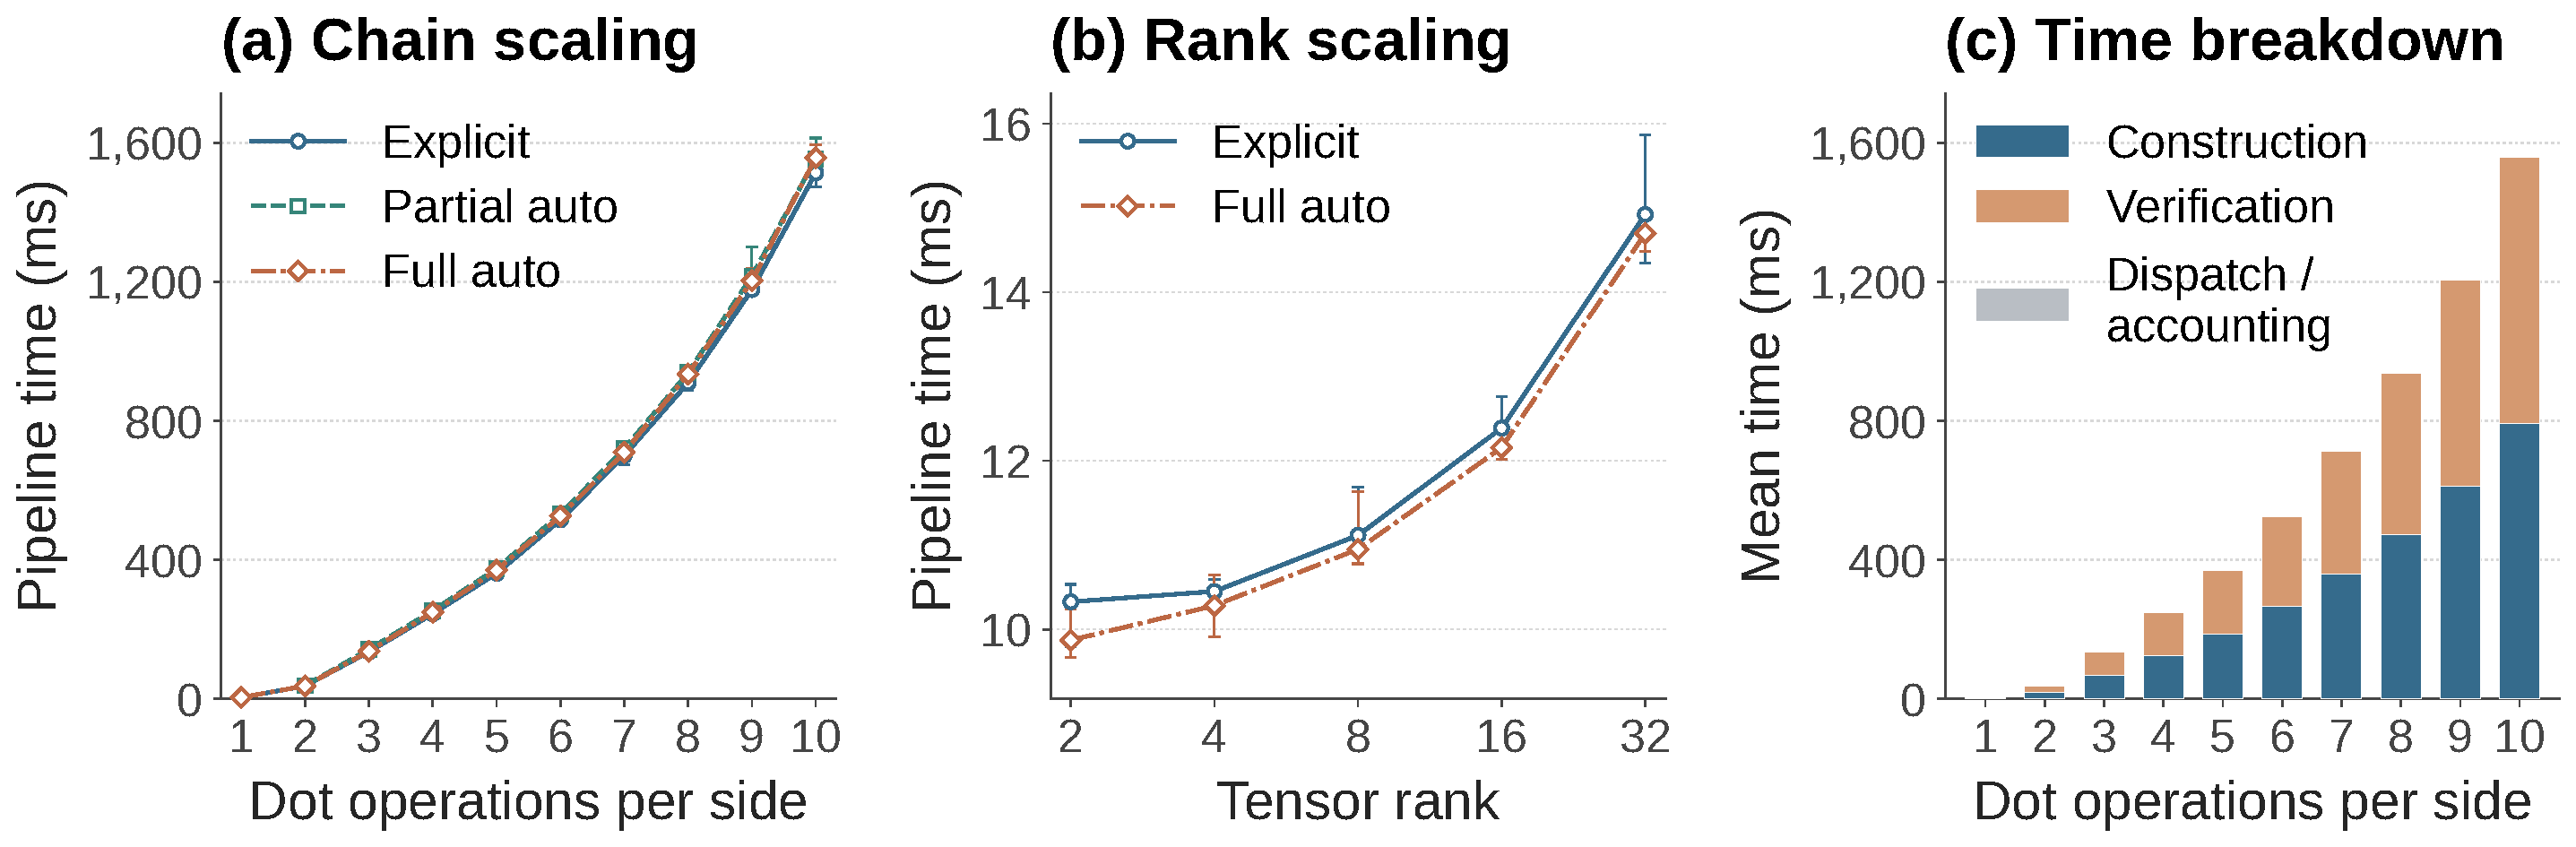
\includegraphics[width=\linewidth]{figures/scalability.pdf}
\caption{Construction and verification scaling: (a)~chains at rank three,
(b)~transpose ranks, and (c)~mean full-auto phase times.
Curves show medians and minimum--maximum whiskers.}
\label{fig:scalability}
\Description{Three panels show pipeline time increasing with the number of
dot operations, a modest increase with transpose rank, and stacked mean
times for construction, verification, and dispatch or accounting.}
\end{figure}

\begin{table}[!htbp]
\caption{Scalability results and their interpretation.}
\label{tab:scalability-results}
\centering
\small
\setlength{\tabcolsep}{4pt}
\begin{tabularx}{\linewidth}{@{}>{\raggedright\arraybackslash}p{0.17\linewidth}YY@{}}
\toprule
Aspect & Result & Interpretation\\\midrule
(a) Chain scaling
& Full-auto median time increases from 0.25~s at 4 dots to 1.56~s at 10 dots.
& Superlinear growth in this interval; no asymptotic bound is established.\\
\addlinespace
(b) Rank scaling
& Full-auto median time increases from 9.87~ms at rank 2 to 14.70~ms at rank 32.
& Rank has a modest effect for symbolic transpose composition.\\
\addlinespace
(c) Time breakdown
& At 10 dots, mean times are 0.793~s for construction and 0.765~s for verification.
& Both phases contribute substantially: approximately 51\% and 49\% of total time.\\
\addlinespace
Tested limits
& All 39 configurations succeed in every measured repetition within the deadline.
& Feasible over the tested range; no failure boundary is identified.\\\bottomrule
\end{tabularx}
\end{table}
\endgroup
\FloatBarrier

\paragraph{Interpretation and measurement limits.}
Figure~\ref{fig:scalability} and Table~\ref{tab:scalability-results} show
comparable total costs for explicit, partial-auto, and full-auto modes.
However, different solver paths mean that differences between their curves
do not directly isolate synthesis overhead.

The evaluation covers canonical contraction chains and symbolic transpose
composition. Larger graphs, other axis layouts, and other operator families
remain untested. Increasing chain length also increases expression depth,
so their effects are not separated. Measurements characterize metadata
reasoning rather than numerical tensor execution or end-to-end compilation.
Finally, five measured repetitions on one machine provide limited evidence
about runtime variability; the plotted minimum--maximum whiskers are not
confidence intervals.
\FloatBarrier
